\chapter{\label{ch:fitting_datasets}Fitting Datasets to the Model}
Recall that the main goal of this work is to investigate pulmonary function of a patient using the Structured Light Plethysmography technique. Now that we have at our disposal a simulation of the human torso with high level controls, we present a data-driven approach to drive the model. For this purpose, we need to adapt the simulation to both the patient's anatomy (by fitting an appropriate skin mesh) and the patient's breathing (by deriving the control parameters from the SLP dataset). To date, only \cite{dilorenzo2009breathing} has proposed a data-driven approach to model the behaviour of actuated physically-based deformable muscles. However, the constraints and hypotheses they use are questionable and will be discussed further in section \ref{sec:fitting}. In addition, there appears to be no previous work related to the fitting of a skin mesh to a particular anatomy in breathing applications.

In section \ref{sec:slp}, we will briefly present the SLP technique and the nature of the data it provides. Section \ref{sec:skin_mesh} will explain how we fit an adapted skin mesh to the model and section \ref{sec:skin_deformation} will describe how this skin mesh is deformed according to the rib cage and abdomen motion. Finally, section \ref{sec:fitting} details the optimisation algorithms used to fit the SLP dataset to the model.

% -------------------------------------------------------------
% Section
% -------------------------------------------------------------
\section{\label{sec:slp}Structured Light Plethysmography datasets}
Structured Light Plethysmography is a non-invasive method for pulmonary function testing using visible light \cite{slp2010}. This technique uses two motion capture cameras and a known grid which is projected onto the chest and abdomen of a patient as figure \ref{fig:slp_device} illustrates.

\begin{figure}
	\centering
	 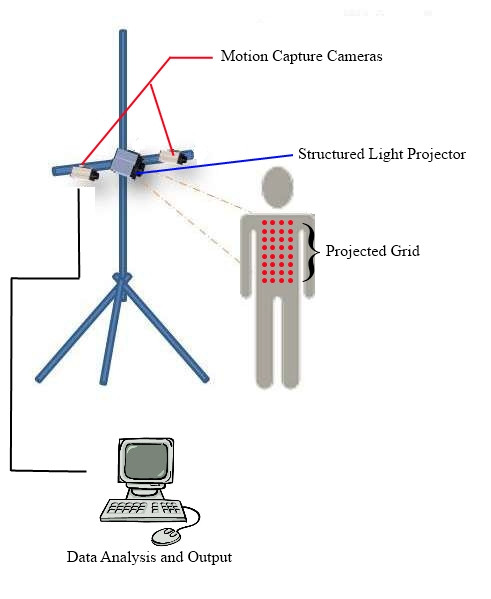
\includegraphics[width=0.7\textwidth]{pics/slp_device}
	\caption[Diagram of the Structured Light Plethysmography device]{\label{fig:slp_device}Diagram of the Structured Light Plethysmography device.}
\end{figure}

It relies on triangulation to reconstruct the space locations of the grid points projected by combining the images of the two cameras for each frame (see figure \ref{fig:slp_reconstruction}). Once the grid points are tracked, put into correspondence and reconstructed, only those on the chest and abdomen areas are retained---this is done by a heuristic procedure \cite{deboer2010breathing}. More details can be found concerning the reconstruction step in the SLP technique in \cite{stuart2011}.

The SLP system ultimately provides us with the space coordinates over time of the grid points that are located on the chest and abdomen of a patient breathing. From the 25x30-point initial grid, a subset of varying size usually from 5x5 to 10x10 is finally retained.

\begin{figure}
	\centering
	 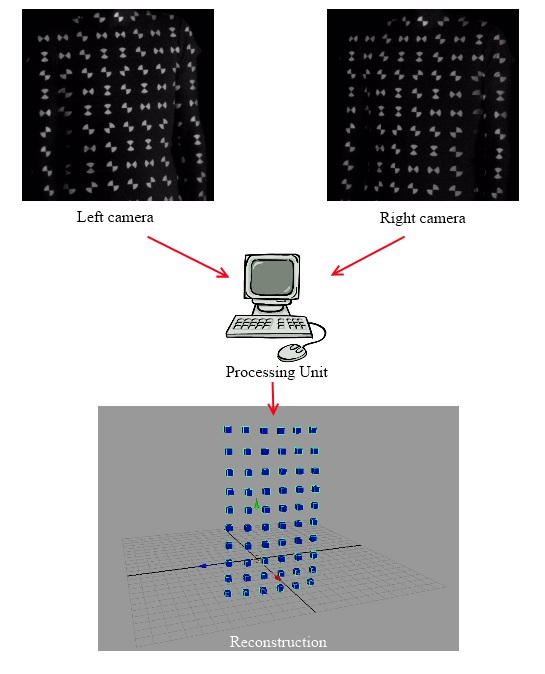
\includegraphics[scale=0.7]{pics/slp_reconstruction}
	\caption[SLP in action]{\label{fig:slp_reconstruction}SLP in action: the images from the left and right cameras are processed to track the grid points which are then put into correspondence and reconstructed.}
\end{figure}

% -------------------------------------------------------------
% Section
% -------------------------------------------------------------
\section{\label{sec:skin_mesh}Adapting a skin mesh}
\begin{figure}
\centering
\subfigure[]{
   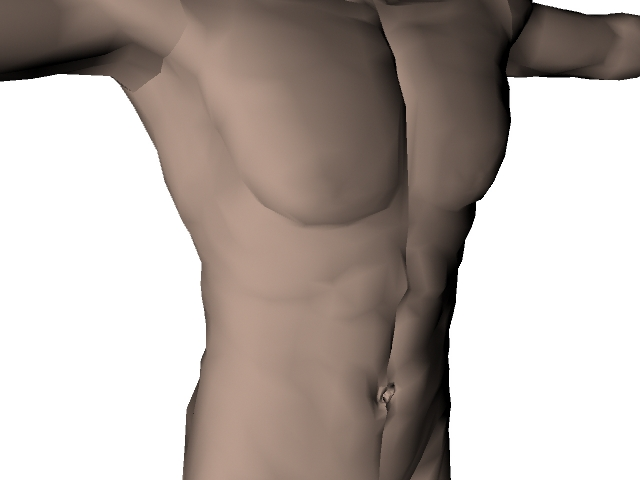
\includegraphics[width=0.3\textwidth]{pics/m_complete_skin} 
\label{fig:1_m_complete_skin}
}
\subfigure[]{
   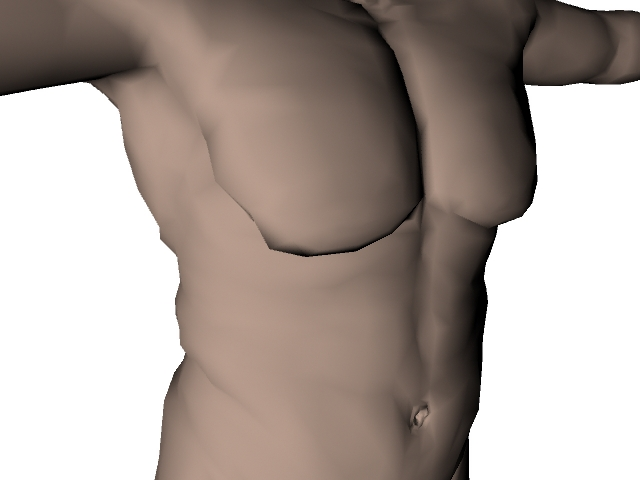
\includegraphics[width=0.3\textwidth]{pics/m_complete_skin_ow}
\label{fig:2_m_complete_skin_ow}
}
\subfigure[]{
   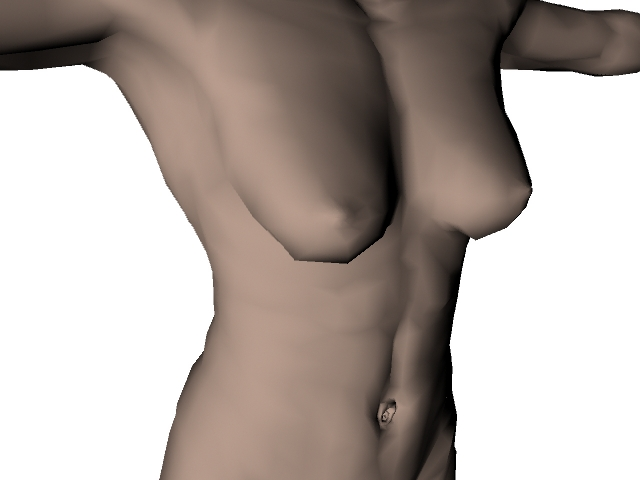
\includegraphics[width=0.3\textwidth]{pics/m_complete_skin_f}
\label{fig:3_m_complete_skin_f}
}
   \caption[Personalised skin meshes derived according to physiognomy data]{Personalised skin meshes derived from Make Human \cite{makehuman2010} according to physiognomy data.
   \subref{fig:1_m_complete_skin} male, 22-year old, 1.75~m, 68~kg, 0~\% breast size.
   \subref{fig:2_m_complete_skin_ow} male, 40-year old, 1.70~m, 80~kg, 0~\% breast size.
   \subref{fig:3_m_complete_skin_f} female, 30-year old, 1.65~m, 55~kg, 80~\% breast size.}
 
   \label{fig:diff_skin}
\end{figure}

In this section we will use a number of 3D computer graphics terms:
\begin{description}
	\item[rigging:] the process of creating the bone structure (also called the skeleton) for a character.
	\item[skinning:] the process of binding a skeleton to a single mesh object.
	\item[skinning deformation:] the process of deforming the mesh as the skeleton is animated or moved.
\end{description}	

In our case, the skeleton is composed of bones (ribs, vertebrae, sternum), a deformable part (the abdomen) and joints linking the bones to each other. Our goal is to fit an adapted skin mesh to this skeleton and deform it as the skeleton moves.

To have a simulation as close as possible to a patient's anatomy, it is crucial to have a skin mesh which closely matches the patient's external shape. In addition, as the SLP only captures the front of the chest wall, the skin mesh and the skinning deformation have to be done with special care, otherwise significant fitting errors would be introduced in the optimisation step.

To help understand the different steps of adapting a skin mesh to a patient, we will use the following real life example for the rest of this section: a subject is asked to breath in different positions in front of an SLP device. The grid is projected so that the first row is aligned with the line defined by the clavicles of the subject; this procedure allows us to have spatial reference points to later place the grid onto the model's skin. The subject is asked to wear a tight T-shirt to avoid skin features and creases which might distort the grid projected by the SLP device. We usually end up with a 6x10 grid over 1000 frames corresponding to about 16.7 seconds and 4 breaths.

From the coordinate matrices the SLP system outputs for the grid points on each frame, we match each grid point of the SLP system to a box marker in the simulation (see figure \ref{fig:slp_reconstruction}). Each marker moves according to the space location of the grid point it is matched to. The first step consists of scaling the model to the SLP scale, or conversely, converting the space coordinates of the SLP reconstructed grid points to the scale of the model. This is trivially done by computing a known distance (for instance between two grid points) on the model and comparing it to the actual distance given by SLP.

From physiognomy data of the patient (gender, age, height, weight, breast size) we derive a skin mesh using the Make Human \cite{makehuman2010} software (see figure \ref{fig:diff_skin}), which is an open source tool for making 3D characters. The skin obtained is generally a good initial fit to the patient's torso as the skin is high resolution (6572 vertices and 19683 edges in total) and the physiognomy parameters sufficiently definite, for a good level of personalisation. The next step is to correctly position the SLP grid onto the skin mesh. The grid is manually placed onto the skin (figure \ref{fig:1_located}) by applying a global rotation and translation matrix to all the grid point coordinates. This is done by aligning the points of the first row of the SLP grid (originally projected on the line defined by the clavicles during the experiments) to the clavicle's line on the skin mesh. We then derive the transformation matrix that we then apply to all grid points. The frame used to initialise the position of the grid on the skin has to correspond to the inflexion point of breathing between expiration and inspiration (when the expansion of the rib cage and the abdominal cavity are minimum). In our example, this frame is conveniently at frame 1.

We compute the error between the skin mesh and the current SLP grid by summing the distances between each grid point and the closest vertex on the skin, this value is then normalised by dividing it with the number of grid points to finally obtain the skin fitting error. In our example, the initial error between the skin and the grid points is 0.5091~cm (see figure \ref{fig:1_error_located_mse=05091}). However, we will now see that this mesh skin can be improved and fitted more precisely to the patient's anatomy.

Even though the skin mesh is composed of many vertices, the distance between a grid point and its associated vertex is still significant---given that we have a mean error of 0.5091~cm and that the actual breathing displacement of the rib cage can be lower than 0.5~cm in the medial direction. Moreover, some points contribute much more in the error function than others (the variance is 0.0329~cm$^2$, see figure \ref{fig:1_error_located_mse=05091}). To lower the error of the skin fitting, our approach was to displace the vertices to the grid point locations they are associated with (see figure \ref{fig:2_vertices_moved}) and then to smooth the whole skin to avoid skinning artefacts; this is done for each dataset even for the same patient (from one experiment to another, there may be movements of the patient that lead to creases of the T-shirt worn and as a consequence to skinning artefacts). The smoothing is done by averaging the values of the five closest vertices for each vertex of the skin mesh (see figure \ref{fig:3_vertices_average}) producing a smoother surface without modifying the topology of the skin. We finally find a much better fit, with a mean skin fitting error of 0.1404~cm and a variance of 0.0038~cm$^2$ (see figure \ref{fig:3_error_vertices_average_mse=01404}).

\begin{figure}
\centering
\subfigure[]{
   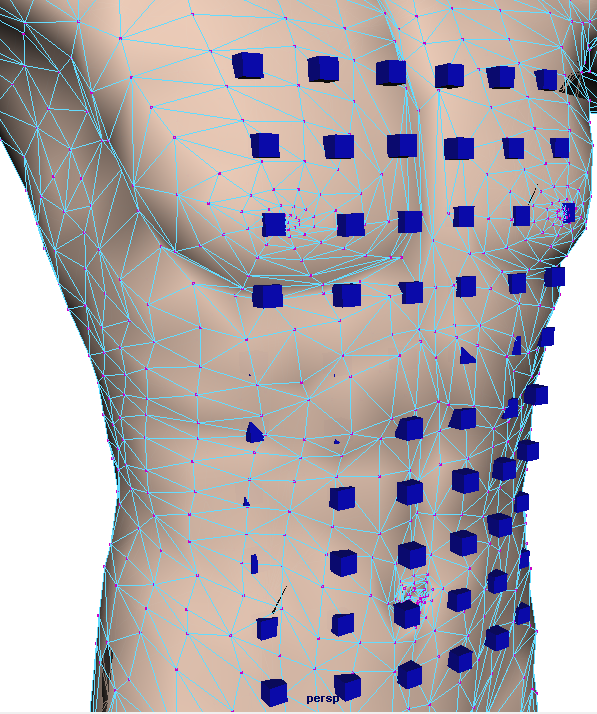
\includegraphics[width=0.3\textwidth]{pics/1_located} 
\label{fig:1_located}
}
\subfigure[]{
   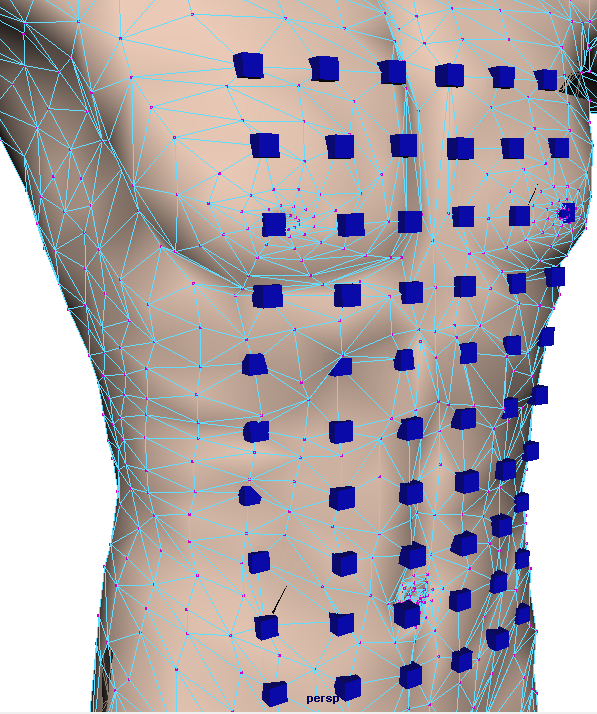
\includegraphics[width=0.3\textwidth]{pics/2_vertices_moved}
\label{fig:2_vertices_moved}
}
\subfigure[]{
   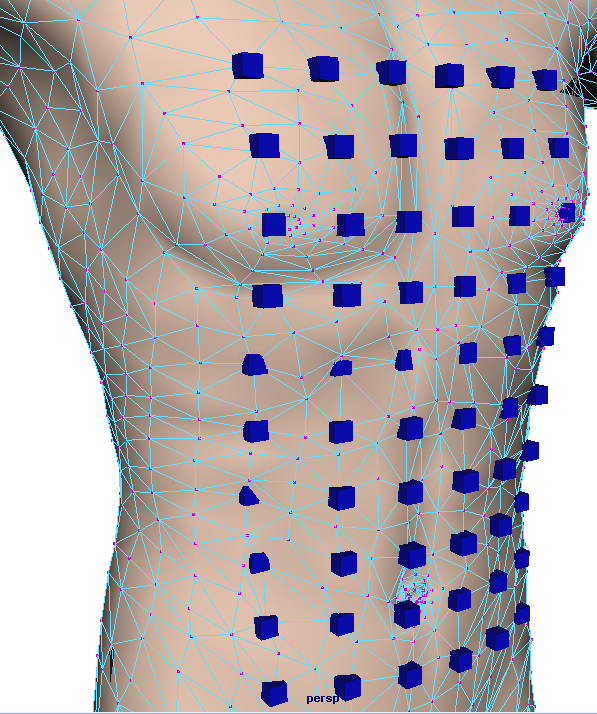
\includegraphics[width=0.3\textwidth]{pics/3_vertices_average}
\label{fig:3_vertices_average}
}
\subfigure[]{
   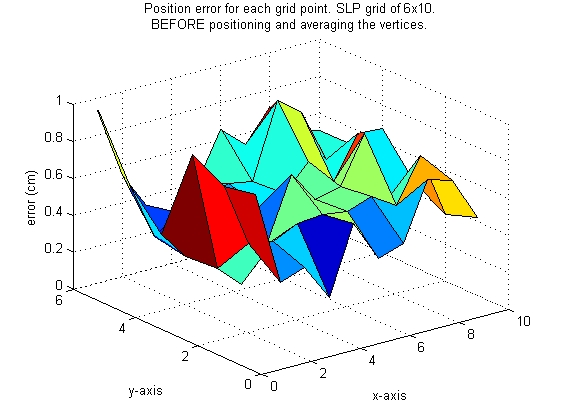
\includegraphics[width=0.45\textwidth]{pics/1_error_located_mse=05091}
\label{fig:1_error_located_mse=05091}
}
\subfigure[]{
   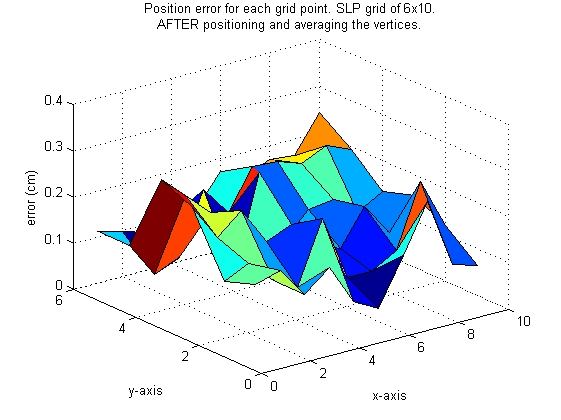
\includegraphics[width=0.45\textwidth]{pics/3_error_vertices_average_mse=01404}
\label{fig:3_error_vertices_average_mse=01404}
}
   \caption[The process of fitting a skin mesh]{The process of fitting a skin mesh.
   \subref{fig:1_located} the SLP grid points are subjected to a global geometric transformation in order to locate them on the initial skin mesh. The frame chosen to initialise the grid corresponds to the inflexion point between inspiration and expiration of the patient. In our example it corresponds to frame 1.
   \subref{fig:2_vertices_moved} each vertex associated with a grid point is moved to the grid point location.
   \subref{fig:3_vertices_average} the skin mesh is then smoothed by averaging each vertex location with its immediate neighbours.
   \subref{fig:1_error_located_mse=05091} the error (z-axis) is plotted for each point of the 6x10-point grid (x-axis and y-axis) with the initial skin mesh at frame 1. The mean error is 0.5091~cm and the variance 0.0329~cm$^2$.
   \subref{fig:3_error_vertices_average_mse=01404} the error (z-axis) is plotted for each point of the 6x10-point grid (x-axis and y-axis) with the new skin mesh (after the vertices were re-positioned and averaged) at frame 1. The mean error is 0.1404~cm and the variance 0.0038~cm$^2$.}
   \label{fig:skin}
\end{figure}

% -------------------------------------------------------------
% Section
% -------------------------------------------------------------
\section{\label{sec:skin_deformation}Skinning deformation}
Once the skin mesh fits the patient's anatomy, it has to deform according to the animation of the underlying skeleton. In most situations, when it comes to skinning deformation problems, the skeleton structure is simpler and made of joints linked with wires referred to as \emph{bones}, this is the so-called rigging process. In our case, the skeleton is more complex as the moving parts of our model are the sternum, the ribs and the abdominal cavity.

The \emph{de facto} standard in real-time algorithms for mesh deformation makes use of a set of per-bone weights associated with each vertex of the skin mesh. Each vertex has a per-bone weight giving a measure in the range $[0, 1]$ of the influence of the particular bone on that vertex. These weights are normalised so that the sum of all per-bone weights for a particular vertex is 1. Traditionally the task of assigning the weights has been done manually and consisted of going through all bones of the skeleton and carefully adjusting the weights with a `weight painting brush' onto the skin mesh. Baran and Popovi{\'c} \cite{baran2007automatic} developed a method, namely \emph{bone heat}, that can automatically derive the skin weights. This technique models weight assignment as a heat diffusion system on the surface of the mesh. For each bone, the vertices which have that bone as their nearest visible bone are initialised to have a surface temperature inversely proportional to the square of their closest distance to the bone. Wareham and Lasenby \cite{wareham2008bone} propose a refinement of \emph{bone heat}, termed \emph{bone glow}, which copes with \emph{bone heat} weaknesses when it comes to assigning weights on surfaces containing creases.
However, as the deformation of the skin implied in breathing does not involve any twisting, creases or any distortion of that type on the skin, we use \emph{bone heat} (available in Maya 2010) for the automatic weight assignment algorithm; the final map representing the weights over the skin mesh in our example can be seen in figure \ref{fig:weights_map}.

\begin{figure}
	\centering
	 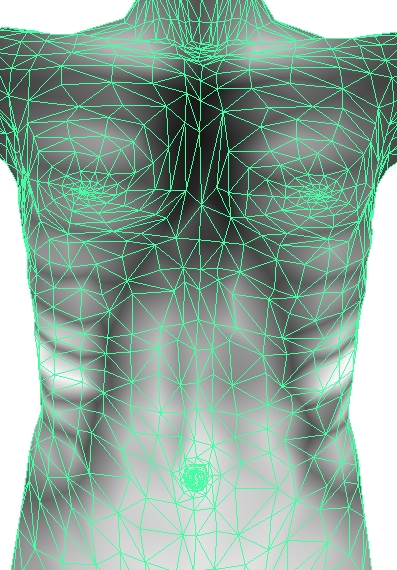
\includegraphics[width=0.5\textwidth]{pics/weights_map}
	\caption[Skin weights of the fitted skin mesh]{\label{fig:weights_map}Skin weights of the fitted skin mesh. Each vertex of the skin is assigned weights that correspond to the influence of the different underlying bones. The sum of the weights assigned to each vertex, defining the influence of the underlying bones onto the skin mesh, has been indicated using a gradation from black to white to represent the range $[0, 1]$.}
\end{figure}

Once the weights for each vertex are assigned, several techniques can be used to deform the skin mesh; the most commonly used is the Linear Blend Skinning (LBS) \cite{lewis2000pose}. LBS consists in deforming vertices as a weighted linear combination of the movement of the bones they are attached to. Some improvements to this algorithm have been designed to cope with artefacts that may appear around joints that are bent or twisted too far. Mohr and Gleicher \cite{mohr2003building} add rotations and scale joints to the skeleton, Kavan et al. \cite{kavan2007skinning} use spherical and dual-quaternion interpolation schemes. However, as the movements in breathing don't involve creases, bends or twists of the skin, the LBS method seemed the most relevant method to apply in our case in terms of computing efficiency and quality of the skinning deformation.

Consequently, at this stage, we have a simulation of the human torso with a skin mesh fitted to a patient's anatomy. This skin mesh is deformed according to the underlying skeleton motion which is driven by the activations of the respiratory muscles.

\begin{figure}
	\centering
	 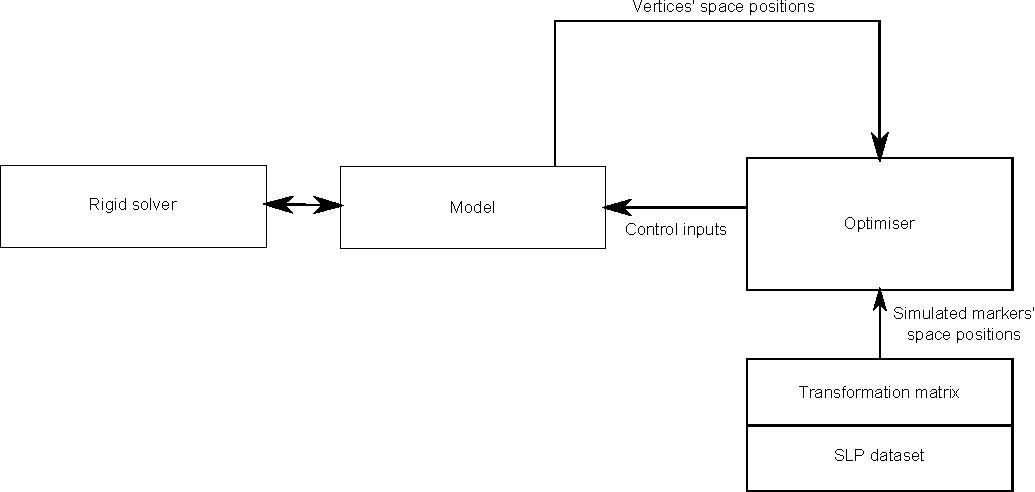
\includegraphics[width=0.8\textwidth]{pics/slp_optim}
	\caption[SLP-driven system overview]{\label{fig:slp_optim}SLP-driven system overview.}
\end{figure}

% -------------------------------------------------------------
% Section
% -------------------------------------------------------------
\section{\label{sec:fitting}Fitting of SLP datasets}
The final phase for generating an animation is the integration of the breath motion data from SLP to our torso simulation. To this end, we explore adaptation methods that employ optimisation techniques to modify a generic model of respiration to fit the breathing patterns and characteristics of specific individuals. Because the datasets given by SLP cannot be directly used to control the simulation, the optimisation attempts to derive the different muscle activations of our simulation to fit a given SLP dataset. 

The SLP-driven system overview can be seen in figure \ref{fig:slp_optim}.

The SLP dataset is fed into the optimiser to determine the best control inputs to feed into the torso simulation. This generates movement from the model that is used to compare to the SLP dataset. The optimiser, iteratively updates the parameters of the control inputs so as to minimise the discrete cost function to produce increasingly better fits of the dataset. We set the cost function to be the error between the human and simulated motion data as:

\begin{equation} \label{eq:cost_fct} f_{error} =  \frac{
\displaystyle\sum\limits_{i=1}^f \displaystyle\sum\limits_{j=1}^p d(i,j)}
{
f \times p
}
\end{equation}

where $ f $ is the number of frames, $ p $ the number of SLP grid points and $ d(i,j) $ the distance between the j-th SLP grid point and its associated vertex on the skin mesh at frame $ i $.

At each step, the optimiser computes the cost function and infers the next set of input parameters. The cost function is derived from the SLP grid point locations (after being geometrically corrected for projection effects through the application of a transformation matrix), and the space positions of the vertices associated with each grid point. The positions of these vertices are computed by the dynamic solver which takes into account the control inputs given by the optimiser and the model. 

As the cost function determination requires a lot of computing power (between 20 and 30 minutes on an Intel(R) Core(TM) i5 CPU for a sequence of 1000 frames), we would like the optimisation algorithm to converge in a small number of iterations. One direct way to achieve this, is to keep the number of parameters to be optimised over reasonably low. The controllers we chose are derived from standard activation sets (see figure \ref{fig:simu_activations}): one for the activation level of the rib cage muscles (the external and internal intercostals and the scalene muscles), another for the diaphragm activation level and a last one for the phase shift of the whole sequence. The breath cycle is derived beforehand by analysing the characteristics of the SLP motion data.

We use the Simplex Down-Hill method designed by Nelder and Mead \cite{nelder1965simplex} to optimise the cost function. For all our simulations, the algorithm converges in less than 60 evaluations of the cost function and we end up with a cost error in the range of $[0.1, 0.5]$~cm.

Table \ref{tab:optim_pos} shows the results of the optimisation process with the same subject breathing in different positions (standing, sitting and lying) and figure \ref{fig:vlungs} gives the derived volume curves of the lungs for the different positions.

\begin{table}[h]
\begin{center}
\begin{tabular}{|c|c|c|c|c|}
\hline
position & $A_{ribs}$ & $A_{diaphragm}$ & iterations & $ f_{error} $ (cm)\\ 
\hline
\hline
 standing & 48 & 50 & 52 & 0.2736\\ 
 sitting & 17 & 57 & 33 & 0.3727\\ 
 lying & 55 & 62 & 51 & 0.3813\\ 
\hline
\end{tabular}
\end{center}
\caption[Control parameters derived from the same subject in different positions]{\label{tab:optim_pos}Control parameters derived from the same subject breathing in different positions. $A_{ribs}$ and $A_{diaphragm}$ correspond to the activation percentage of the maximum reachable activations of the ribs muscles and the diaphragm respectively.}
\end{table}

\begin{figure}
	\centering
	 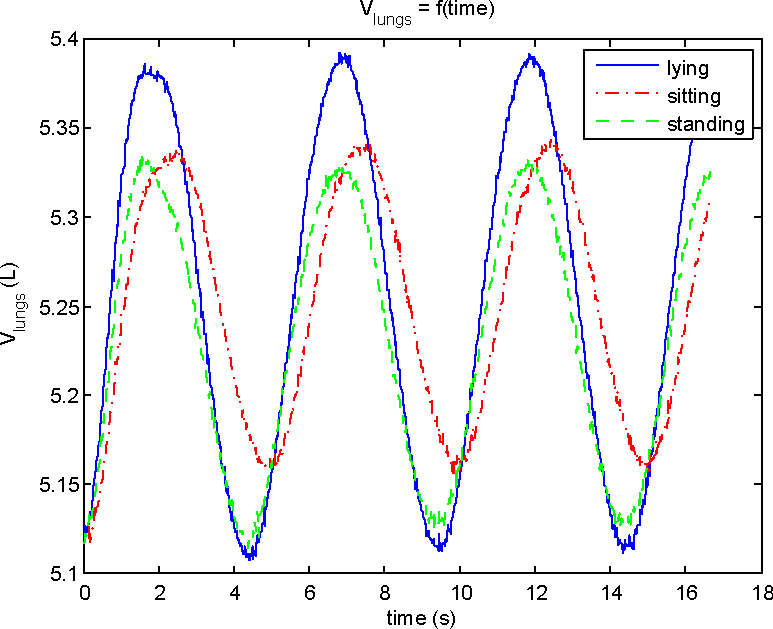
\includegraphics[scale=1]{pics/vlungs}
	\caption[Simulated lungs' volume for the same subject breathing in different positions]{\label{fig:vlungs}Volume of the lungs derived from the simulation of the same subject breathing in different positions.}
\end{figure}